\section{P2 results: working-point outcome, signal efficiency and fallback limits}\label{sec:results}

This section reports the detector-level outcome of the frozen rule, the signal efficiencies and the fallback limits. All
numbers are from the final, frozen analysis run (campaigns C1a, C1b, C2B and A2FC; \rep{acts/stage4/STAGE4_RESULTS.md},
machine-readable in \rep{data/acts_stage4/analysis/STAGE4_SUMMARY.json}). Everything is detector-level simulation in a
public-geometry model, barrel only; the acceptance factor is truth level.

\subsection{Working-point outcome}\label{sec:results:wp}
\textbf{No working point exists in either category.} $\Nbkgeightyfour>0.11$ already at R01 and at every rung after it;
the minimum is $1.23\times10^6$ at R09 in SR-T and SR-G (Section~\ref{sec:bkg:ladder}), and the best fallback column
(FB3) has $2.0\times10^6$ per category, $\approx4\times10^6$ combined, 7.1 decades above 0.3. By the frozen rule the
pre-defined fallback of Section~\ref{sec:strategy:fallback} therefore applies at every $(\mQ,\Lam)$: one admissible
selection per hypothesis, chosen from the frozen admissibility table and never optimised, with a non-zero log-normal
background. The fallback gives efficiencies, backgrounds and expected limits; it gives no background-free statement, no
discovery reach and nothing in the merged regime. Because the deep-rung backgrounds are zero-count bounds
(Section~\ref{sec:bkg:ladder}), the limits below measure the reach of this simulation set-up. They are conservative
with respect to simulation statistics and would move in proportion to the bounds with more simulated events, but the
untested rung factorisation (Section~\ref{sec:bkg:closure}) can bias them in either direction.

\subsection{Signal efficiency}\label{sec:results:eff}
The efficiency counts an event if a candidate passes the selection, has $f_{\rm CKF}<0.2$ and is signal-matched by the
pre-declared definition of Section~\ref{sec:strategy:trig}; the denominator is the template half with $|\eta_{\rm
pair}|<2.5$, 180--200 events per point. The barrel-only selection caps it at $\approx0.3$.

\paragraph{Finder efficiency without pile-up (V4-3: partial).} The pre-registered check V4-3 asked for a finder efficiency
$\ge0.9$ at 1--5\,keV without pile-up. With pairs in the barrel ($|\eta_{\rm pair}|<1$) and a match ``some candidate holds
$\ge50\%$ of the quirk hits'' that was defined only after the first comparison failed (a post-hoc reading), the finder
reaches 0.90--0.97 at 1.5--2\,keV for all five (species, mass) points ($\Etil$ 500: 2\,keV only), but 0.75--0.90 at 1\,keV, 0.83--0.97 at 3\,keV and
0.58--0.84 at 5\,keV; with the counting rung R04 also required it is 0.64--0.77 at 1.5--2\,keV. V4-3 is therefore
\emph{partial}. The losses are understood: R04 needs two crossings on every one of the seven IT and PS barrel layers, so a
single merged pair kills it at high $\Lam$; the seed needs an opening of at least 1\,mrad; and the CKF removes quirk hits.

\paragraph{Efficiency at pile-up 200.} Figure~\ref{fig:eff} shows the efficiency at the fallback selection $r_{\rm fb}$
and along the ladder. At R04 it is 0.085--0.31 at $1$--$5\keV$; at the fallback it is 0--0.080 over all 40 points (maximum
0.080 at $E$ 500 at 2 and $5\keV$ and $\Etil$ 500 at $5\keV$), and zero in both categories at seven points ($E$
500/1000/1500 at $0.45\keV$, $E$ 1500 at $0.6\keV$, $\Etil$ 500 at $\le0.85\keV$). The SR-T share is typically 30--70\% (range 0--100\%) of
$\Eff(r_{\rm fb})$ at $\mQ\ge500\GeV$ and $\le27\%$ at $200\GeV$. At $\Lam\gtrsim2\keV$ the efficiency with pile-up is
\emph{above} the one without: pile-up hits complete the layer count where the quirk pair has merged, so the high-$\Lam$
candidates are partly pile-up-assisted.

\paragraph{Full-chain revert and its systematic.} The fast signal path digitises quirk hits outside ACTS and never passes
them through the CKF. Under the pre-registered rule, the nine points where more than 5\% of quirk hits were taken by CKF
tracks without pile-up ($\{E\,200,500,1000,1500\}\times\{3,5\}\keV$ and $\Etil$ 500 at $5\keV$) were re-run through the
full chain (A2FC; same rows and seeds, pile-up measurement noise re-drawn). At R04, the only genuinely paired rung, the full
chain is 5--30\% lower; summed over eight of the nine points the loss is $\times0.83$ at R04 (84 against 20 discordant
events, $p\approx1.6\times10^{-10}$) and $\times0.87$ at $r_{\rm fb}$, attributed to CKF hit stealing (confirmed for one
event, inferred for the aggregate). At $E$ 500, $3\keV$ the full chain cut $\Eff$(FB3) from 0.145 to 0.055 ($11/200$, 68\%
CP $[0.039,0.076]$); the investigation found no bug and attributes the drop to statistics, because re-drawing the noise
flips 25--50\% of the passing events at R08--R14 (global $p\approx10^{-4}$--$10^{-3}$; a conclusion by exclusion). The full
chain is the reference at the nine points; the 31 others stay on the fast path and may overestimate $\Eff$ by up to
$\approx1/0.87$ (\EST{}, not applied).

\begin{figure}[htbp]
\centering
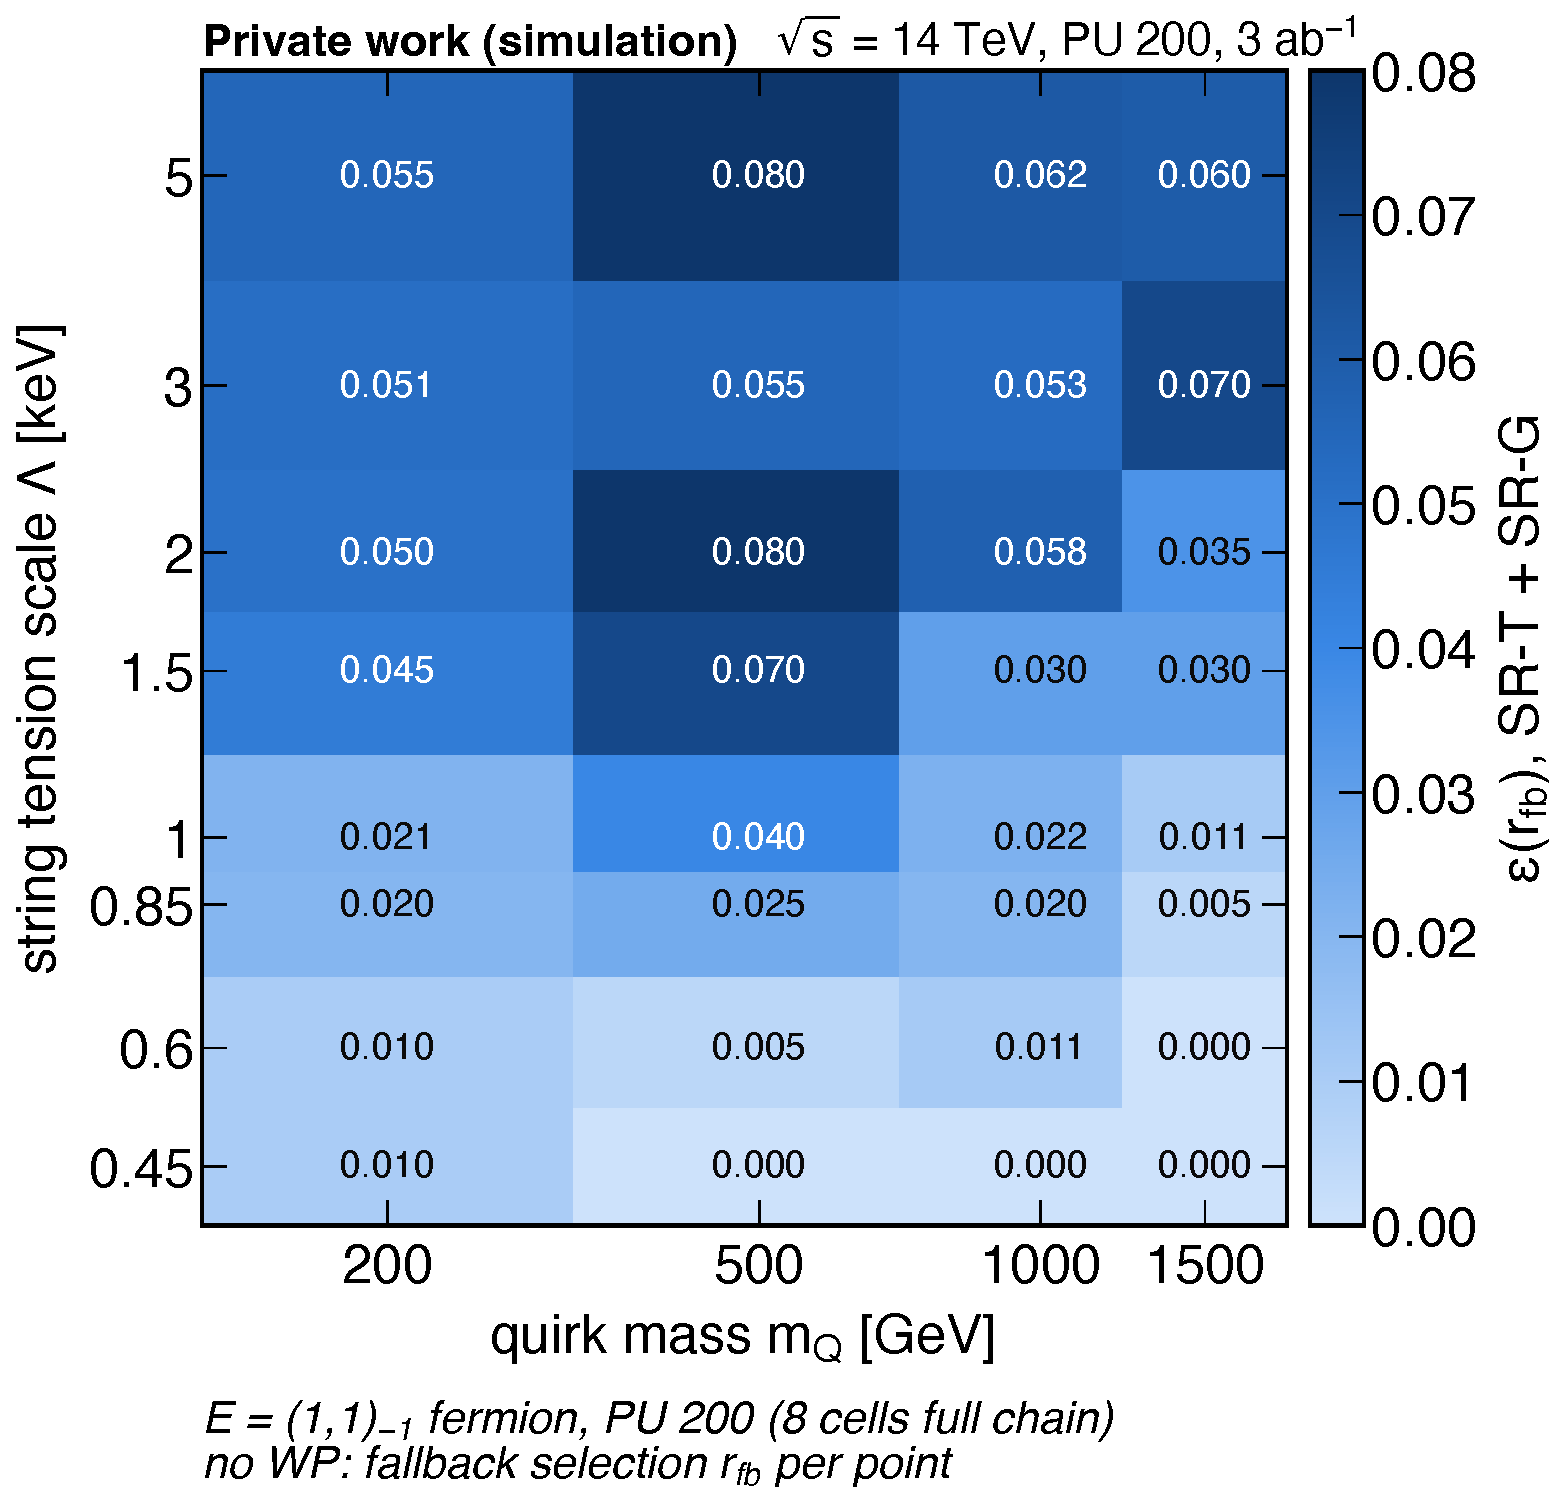
\includegraphics[height=0.37\linewidth]{figures/D1_eps_map_rfb.pdf}\hspace{0.02\linewidth}
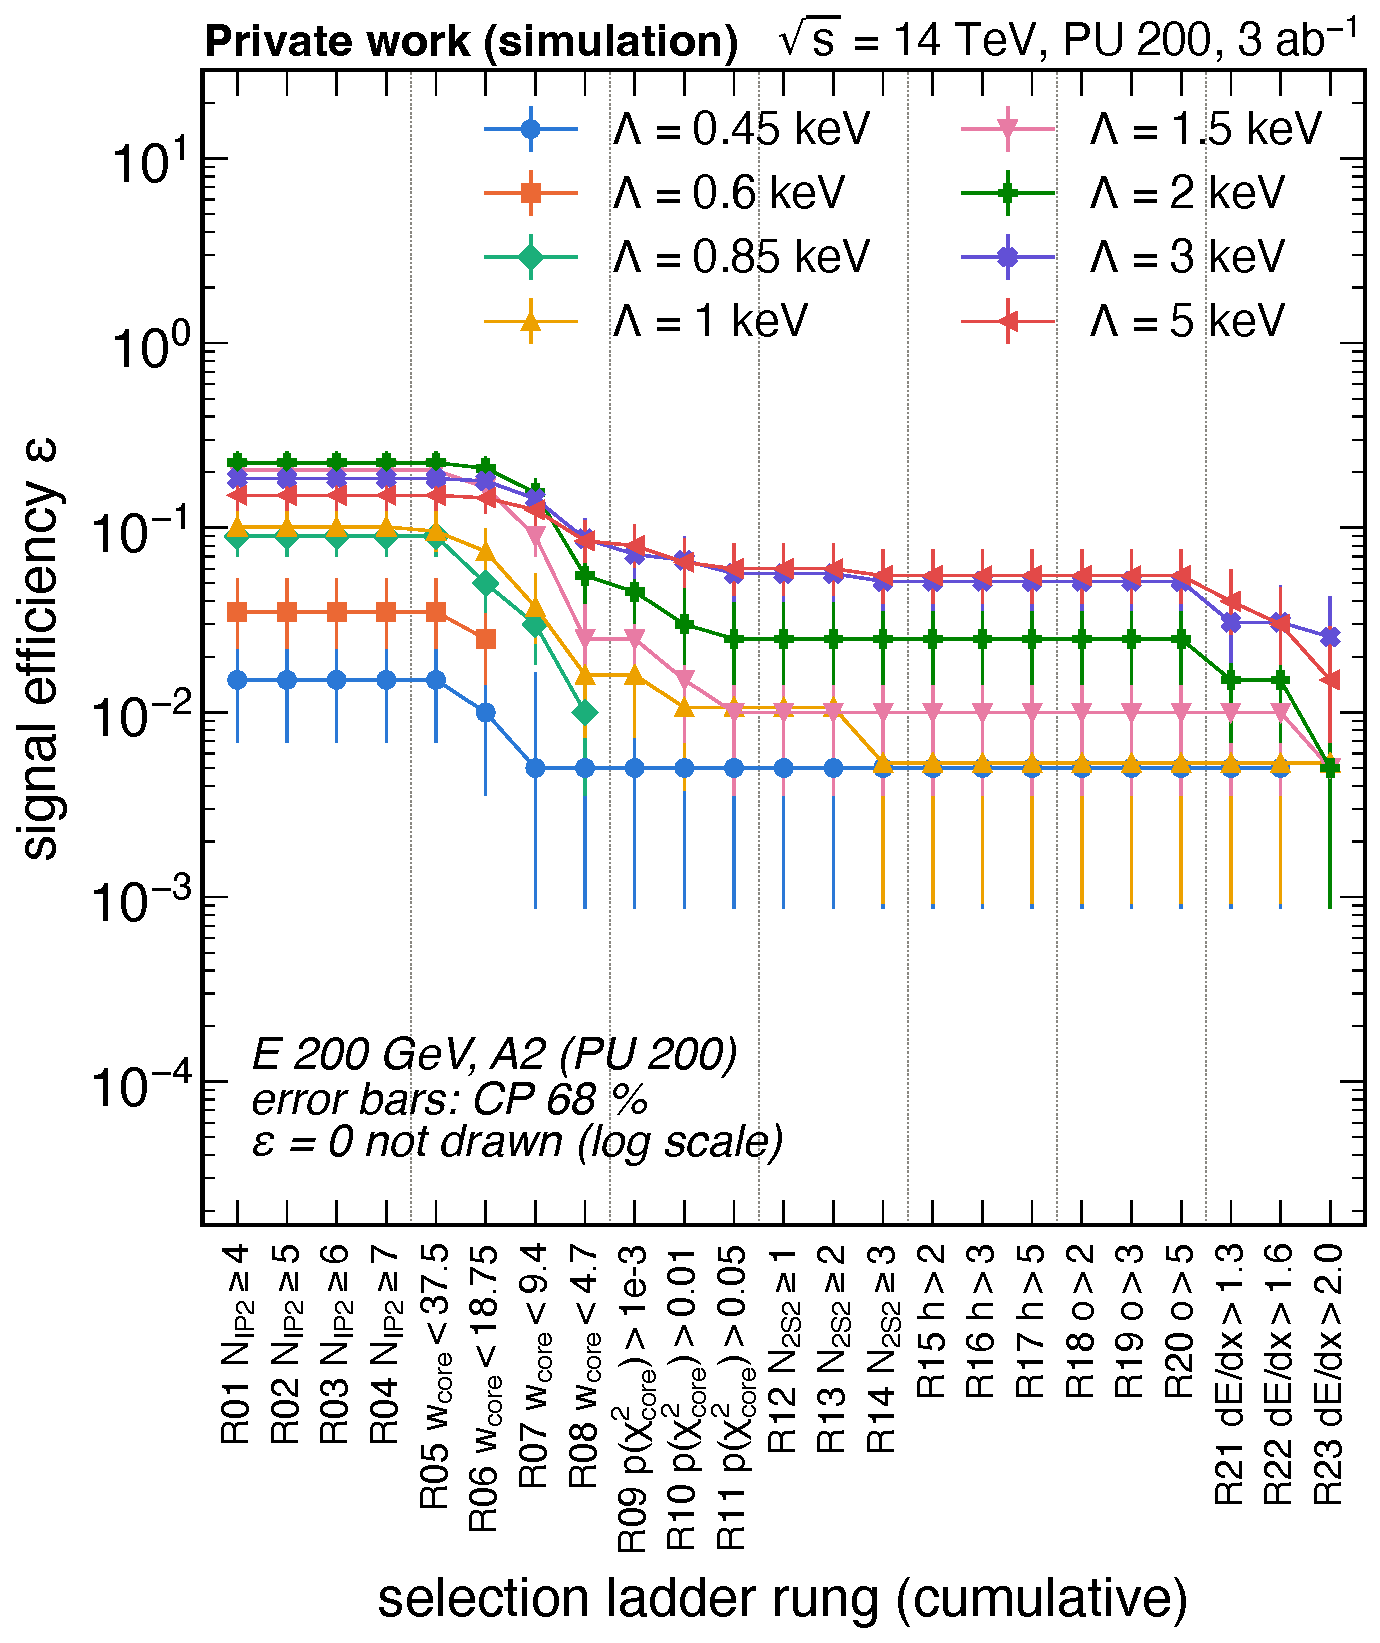
\includegraphics[height=0.37\linewidth]{figures/D2_eff_vs_rung_F200.pdf}
\caption{Signal efficiency at detector level (PU 200, barrel, fermion $E$). (Left) Efficiency at the pre-declared fallback
selection $r_{\rm fb}$ (SR-T + SR-G) on the $(\mQ,\Lam)$ grid; eight cells at 3 and $5\keV$ use the full ACTS chain
(the ninth full-chain point, $\Etil$ 500 at $5\keV$, is not in this map), the others the fast signal path. (Right) Efficiency along the 23 cumulative rungs for $\mQ=200\GeV$ at each $\Lam$, with
68\% Clopper--Pearson errors (zero values not drawn). The efficiency stays below $\approx0.08$ at the fallback: the
barrel selection caps it at $\approx0.3$ and the deep cuts cost the rest.}
\label{fig:eff}
\end{figure}

\subsection{Fallback limits}\label{sec:results:limits}
The expected 95\% CL upper limit on the number of signal events in the trigger and preselection acceptance uses the
two-category counting likelihood of Section~\ref{sec:strategy:fallback} with hybrid-CL$_s$ toys (primary). It is
converted to a limit on the inclusive cross section, $\sigma_{95}=\mu_{95}/(Lf_{200}A)$, with the tail fraction $f_{200}$
and the truth-level acceptance $A$ of Eq.~\eqref{eq:effchain} (Table~\ref{tab:acc}), and compared with
$N_{\rm exp}=\sigma_{\rm norm}f_{200}LA$, so that $\sigma_{95}/\sigma_{\rm norm}=\mu_{95}/N_{\rm exp}$.
Figure~\ref{fig:limits} shows the limits for $\mQ=200\GeV$ against $\Lam$ and against $\mQ$ at $\Lam=1.5\keV$, and
Figure~\ref{fig:excl} in Section~\ref{sec:bounds} the full grid.

\textbf{No point is excluded.} The best expected limit is $\sigma_{95}/\sigma_{\rm norm}=\mu_{95}/N_{\rm exp}=790$ at $E$
200, $\Lam=1.5\keV$ ($r_{\rm fb}=$ FB2, $\Eff=9/200=0.045$, 68\% CP $[0.030,0.065]$, 95\% CP $[0.021,0.084]$; $\mu_{95}=1.25\times
10^7$ events, toy $\pm1\sigma$ band $[8.6\times10^5,1.9\times10^8]$, asymptotic/toys 1.05; $N_{\rm exp}=1.58\times10^4$,
$S=710$, $\sigma_{95}=1.7\times10^5\fb$ against $\sigma_{\rm norm}=219\fb$). The statistical uncertainty of $\Eff$ moves the
ratio by a factor $\approx1.5$ either way at 68\% CL; even the 95\% CP upper efficiency gives $\approx420$, and an
exclusion would need $\Eff\approx36$, which is impossible. With the full-chain systematic of Section~\ref{sec:results:eff}
the ratio becomes $\approx910$--950 (\EST{}, not applied). The second-best point is $E$ 200 at $2\keV$ (820); all others lie
between $2.3\times10^3$ ($E$ 200, $1\keV$) and $6.0\times10^7$ ($E$ 1500, $0.85\keV$). The best ratio per mass is
$1.3\times10^4$ ($E$ 500), $3.8\times10^5$ ($E$ 1000), $3.8\times10^6$ ($E$ 1500) and $2.8\times10^5$ ($\Etil$ 500), all at
$3\keV$; 33 of 40 points have a limit and seven have $\Eff=0$. Even with zero background only 20 of the 40 points would
have $S\ge3$ selected events ($E$ 1500 at most 0.3). The $5\sigma$ discovery yields, where computed, are
$1.9\times10^4$--$2.4\times10^8$ times the prediction. These ratios include $f_{200}$; an earlier version of the
analysis omitted it and quoted values $1/f_{200}=6$--21 times smaller (erratum in \rep{STAGE4_RESULTS.md}).

\begin{table}[htbp]
\centering
\small
\caption{Tail fraction $f_{200}$, truth-level acceptance of the tail sample (Stage 3, template half) and predicted yield
$N_{\rm exp}=\sigma_{\rm norm}f_{200}\,3\abinv\,A$ ($N_{\rm IC}=2$), used to convert the detector-level limits
(\rep{STAGE4_RESULTS.md} \S4.4); $A_{\rm incl}=f_{200}A$. $\Eff_{\rm PV}=1$ (not modelled).}
\label{tab:acc}
\begin{tabular}{lccccccl}
\toprule
point & $f_{200}$ & $\Eff_{\rm fid}$ & $\Eff_{\rm trig}$ & $\Eff_{\rm presel|trig}$ & $A$ & $A_{\rm incl}$ & $N_{\rm exp}$\\
\midrule
$E$ 200 & 0.0476 & 0.847 & 0.90--0.91 & 0.65--0.66 & 0.49--0.50 & 0.024 & $1.55$--$1.58\times10^4$\\
$E$ 500 & 0.104 & 0.830 & 0.92--0.93 & 0.74--0.75 & 0.57 & 0.059--0.060 & $1.08$--$1.09\times10^3$\\
$E$ 1000 & 0.146 & 0.816 & 0.93--0.94 & 0.84--0.85 & 0.64--0.65 & 0.093--0.095 & 55--56\\
$E$ 1500 & 0.169 & 0.752 & 0.94--0.95 & 0.81--0.82 & 0.58 & 0.098--0.099 & 4.2\\
$\Etil$ 500 & 0.1135 & 0.826 & 0.93 & 0.71--0.72 & 0.55 & 0.062--0.063 & 85--86\\
\bottomrule
\end{tabular}
\end{table}

\begin{figure}[htbp]
\centering
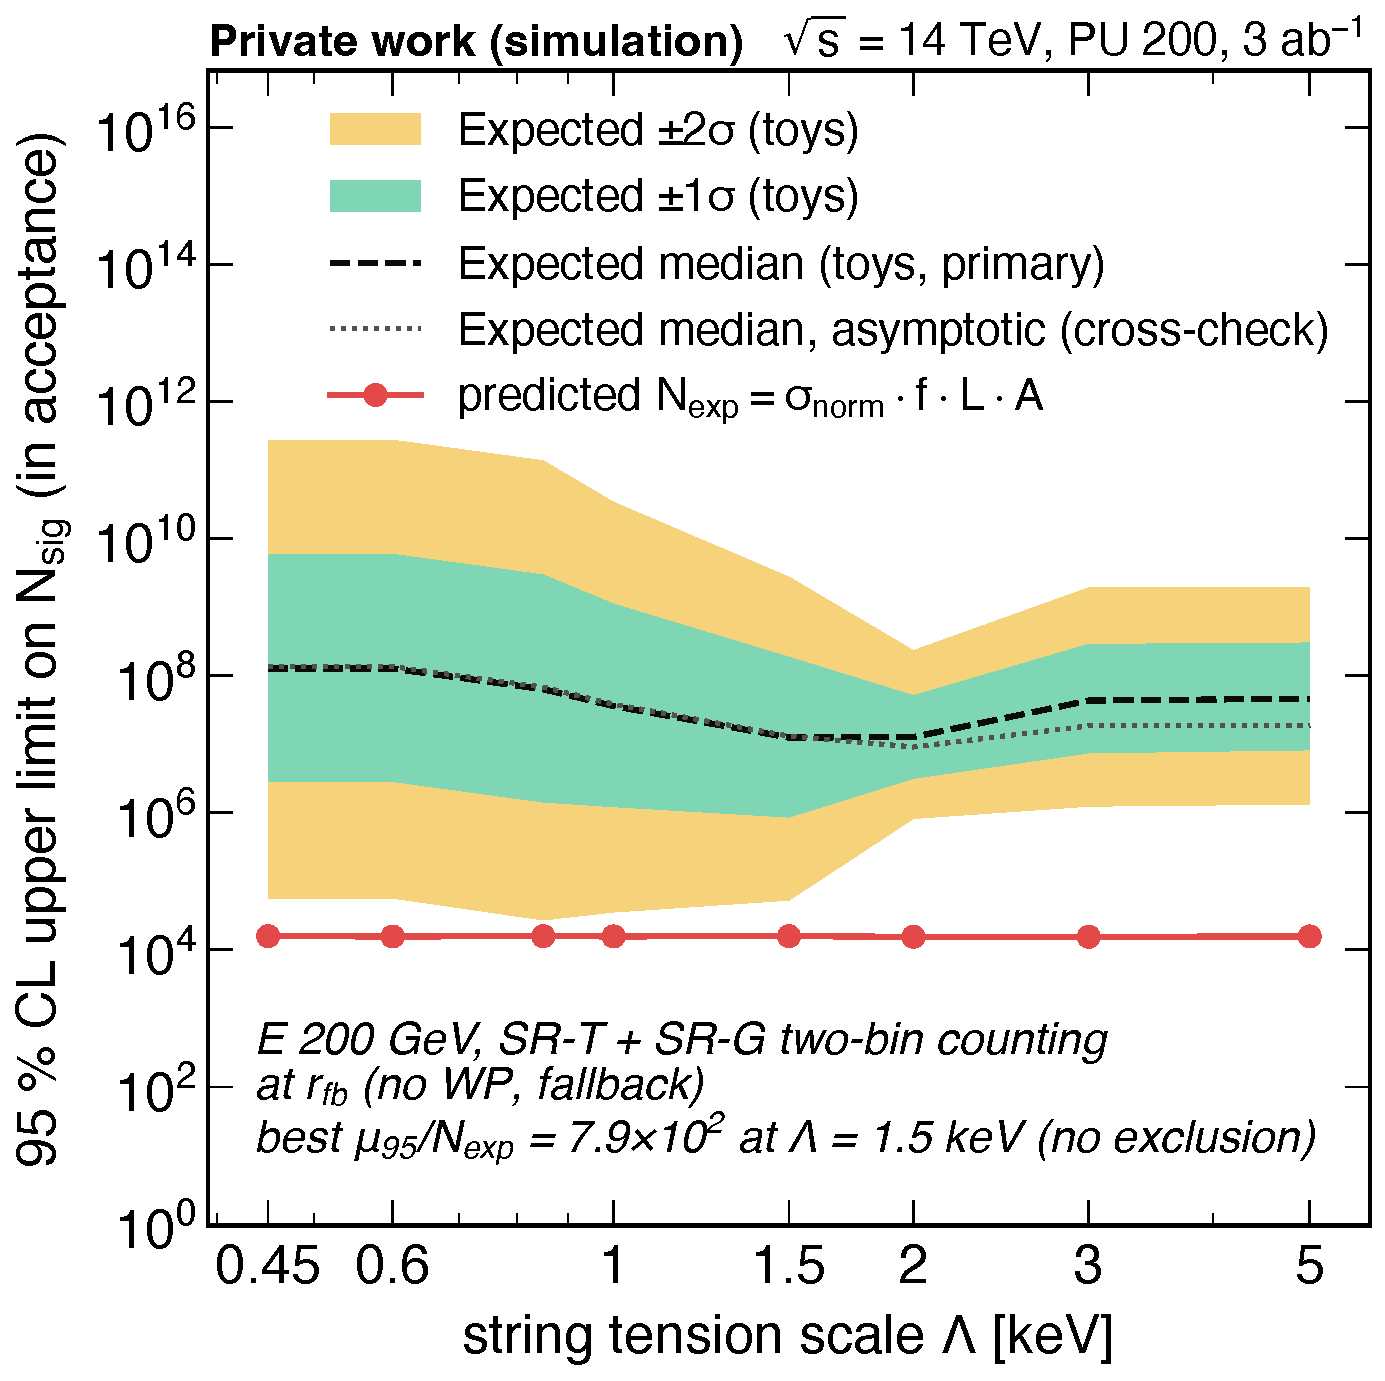
\includegraphics[height=0.37\linewidth]{figures/D5_limit_mu_vs_lambda_F200.pdf}\hspace{0.02\linewidth}
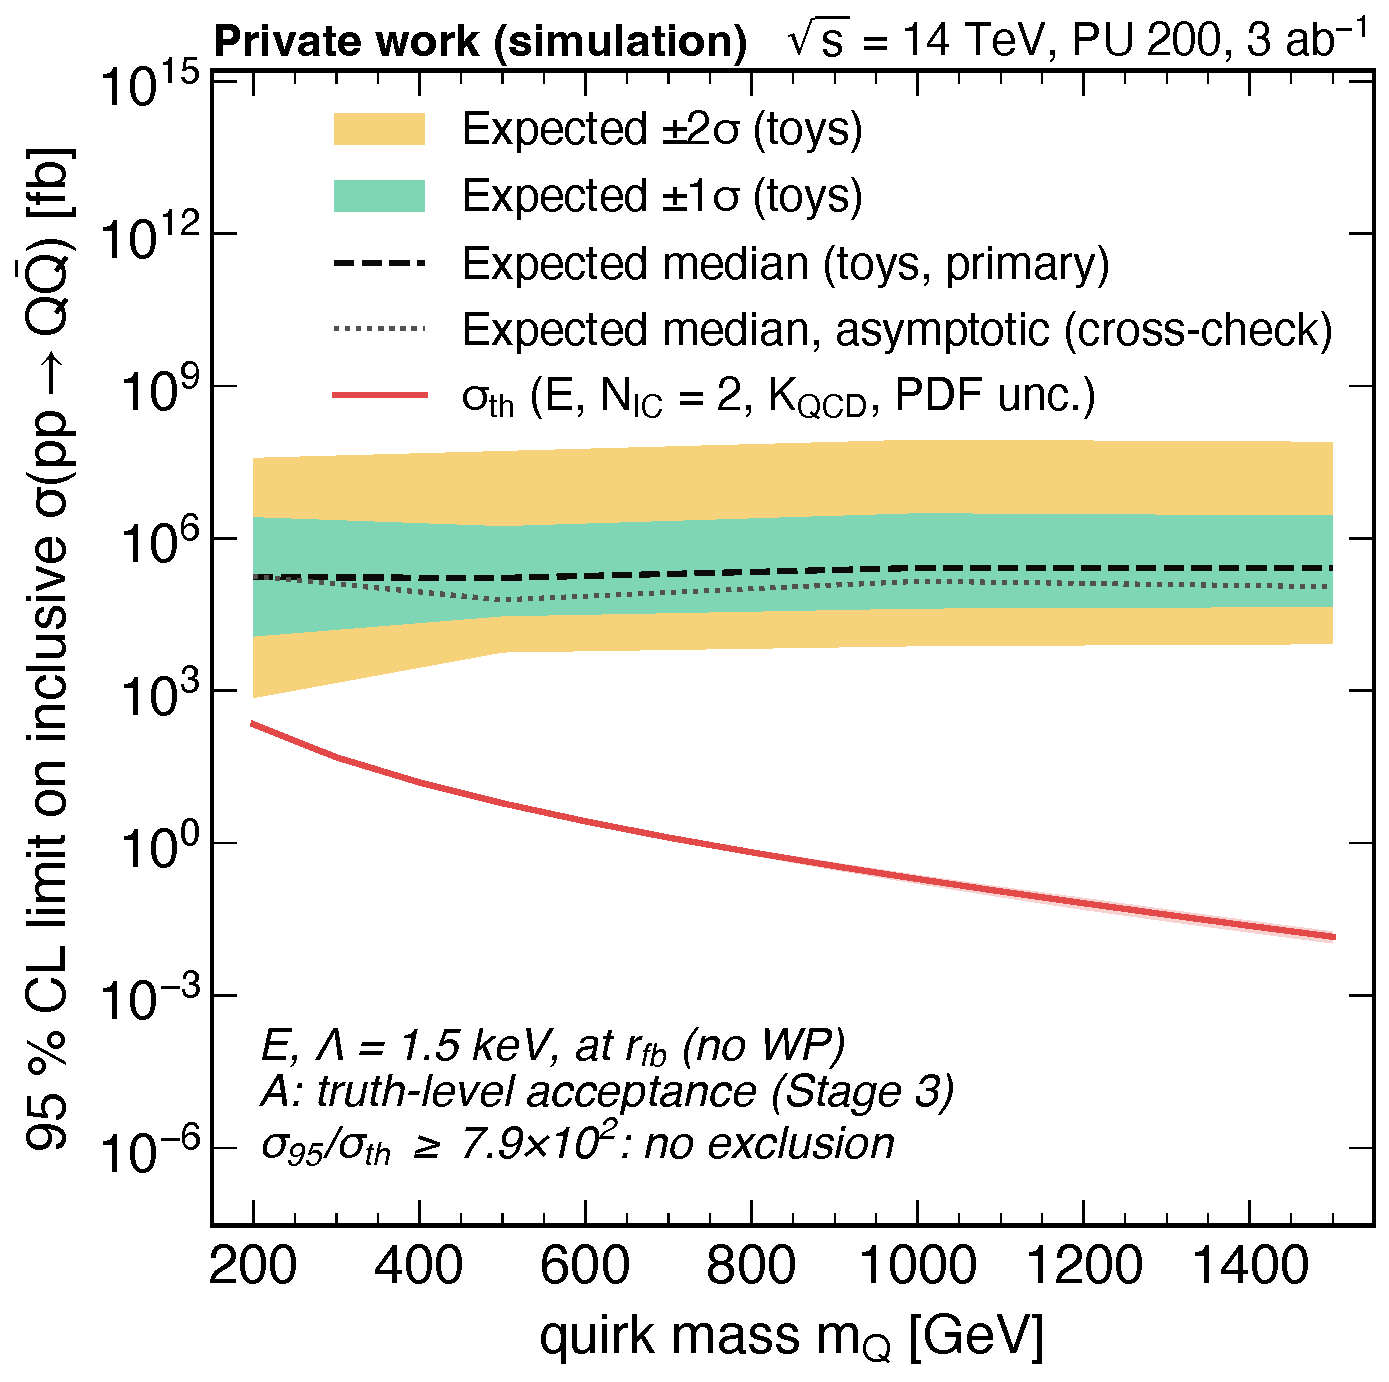
\includegraphics[height=0.37\linewidth]{figures/D6_limit_xsec_vs_m_L1p5.pdf}
\caption{Expected 95\% CL limits at the fallback selection (detector level; acceptance truth level; no working point).
(Left) Limit on the number of signal events in the acceptance for $E$ at $200\GeV$ against $\Lam$, with toy $\pm1\sigma$ and
$\pm2\sigma$ bands (primary), the asymptotic median (cross-check) and the predicted yield. (Right) Limit on the inclusive cross section
against $\mQ$ at $\Lam=1.5\keV$ with the predicted cross section ($\sigma_{\rm norm}$ with $K_{\rm QCD}$, labelled $\sigma_{\rm th}$; $N_{\rm IC}=2$). The median limit is at least 790 times
the prediction everywhere: nothing is excluded. The deep-rung background central values are zero-count simulation bounds.}
\label{fig:limits}
\end{figure}

\subsection{Systematic uncertainties}\label{sec:results:syst}
The limits carry the following uncertainties, each entering as a log-normal nuisance or, where stated, only as a
reported variation. (i) \emph{Signal normalisation}: $\pm5\%$ on $\sigma_{\rm norm}$ (Section~\ref{sec:model:xsec}) and
$+12$--15\%/$-11$--13\% on the tail fraction $f_{200}$ (Section~\ref{sec:model:syst}); neither is propagated into
$\mu_{95}/N_{\rm exp}$, and both are small against the factor $\ge790$.
(ii) \emph{Background}: per term, statistical, extrapolation-model, density-normalisation and normalisation components
(Section~\ref{sec:strategy:rule}); at the headline point the SR-G background is dominated by the zero-count PV-pair bound with
$\sigma_{\ln}\approx1.5$. (iii) \emph{Efficiency}: the binomial uncertainty above and the full-chain systematic (not
applied). The MET resolution (25\,GeV, variations 15/35\,GeV), the trigger turn-on ($\pm25\GeV$ on its 50\% point) and
the PV-identification efficiency are parametrised assumptions (\UNV{}) and are not propagated to the final limits.
(iv) \emph{Statistical treatment}: SR-T and SR-G are treated as uncorrelated although single-interaction and SM terms
enter both identically. This is anti-conservative where both categories carry signal (23 of the 33 points with a limit),
but irrelevant at the headline point, where the SR-T efficiency is zero. None of these can
turn the null result into an exclusion: that would need a background lower by many orders of magnitude.
